% Déclaration de la classe du document (article, report, book, etc.)
\documentclass[12pt, a4paper]{article}

% --- PAQUETS UTILISÉS ---

% Pour gérer l'encodage des caractères, indispensable pour les accents
\usepackage[utf8]{inputenc}

% Pour la gestion de la langue française (césure, typographie, etc.)
\usepackage[french]{babel}
\usepackage{graphicx}
\usepackage{float}
% Pour gérer les marges du document
\usepackage[top=2.5cm, bottom=2.5cm, left=2.5cm, right=2.5cm]{geometry}

% Pour avoir des liens cliquables dans le PDF (table des matières, références)
\usepackage{hyperref}
\hypersetup{
    colorlinks=true,
    linkcolor=blue,
    filecolor=magenta,      
    urlcolor=cyan,
}

% --- INFORMATIONS DU DOCUMENT ---

\title{Rapport de Projet : Cryptohack}
\author{Victor \and Seb}
\date{\today} % Affiche la date de compilation

% --- DÉBUT DU DOCUMENT ---

\begin{document}

% Crée la page de titre à partir des informations ci-dessus
\maketitle

% Génère la table des matières
\tableofcontents

\newpage % Commence le contenu sur une nouvelle page

% --- CONTENU DU RAPPORT ---

\section{Introduction}

\subsection{Contexte du projet}

Ce rapport présente une série de challenges de cryptographie réalisés sur la plateforme CryptoHack. L'objectif est de documenter les approches méthodologiques et les solutions techniques que nous avons mis en oeuvre en binome pour résoudre les défis proposés. En préambule, il convient de situer le contexte de ce travail en présentant d'une part le rôle fondamental de la cryptographie en cybersécurité, et d'autre part l'intérêt des plateformes de type \textit{Capture The Flag} (CTF) comme outil d'apprentissage.

\subsection{Place de la cryptographie en cybersécurité}

La cryptographie est une discipline scientifique qui constitue l'un des piliers de la sécurité des systèmes d'information. Son objet est de développer des techniques permettant de protéger l'information contre toute modification ou accès non autorisé. En cybersécurité, la cryptographie vise à garantir plusieurs principes de sécurité fondamentaux.

\paragraph{La confidentialité}
Ce principe assure que seules les entités autorisées puissent accéder aux données. L'outil principal pour atteindre cet objectif est le chiffrement, qui consiste à transformer une information (le texte clair) en une forme inintelligible (le texte chiffré) à l'aide d'une clé secrète.

\paragraph{L'intégrité}
Ce principe garantit que les données n'ont pas été altérées ou corrompues, que ce soit de manière accidentelle ou intentionnelle, durant leur stockage ou leur transmission. Les fonctions de hachage et les codes d'authentification de message (MAC) sont des mécanismes cryptographiques courants pour vérifier l'intégrité.

\paragraph{L'authenticité}
Ce principe permet de vérifier l'identité d'une entité (un utilisateur, un serveur, etc.). Les certificats numériques et les signatures numériques sont des exemples de techniques cryptographiques assurant l'authentification.

\paragraph{La non-répudiation}
Ce principe empêche une entité de nier avoir effectué une action, comme l'envoi d'un message ou la validation d'une transaction. La signature numérique est le mécanisme de base pour fournir cette garantie.\\

De la sécurisation des communications sur Internet (protocoles TLS/SSL) à la protection des données stockées, en passant par la sécurisation des transactions financières et la protection de la vie privée, les applications de la cryptographie sont omniprésentes et critiques. L'étude de ses mécanismes et de leurs implémentations est par conséquent essentielle pour tout praticien de la cybersécurité.

\subsection{Les plateformes de CTF dans l'apprentissage}

Les challenges de type \textit{Capture The Flag} (CTF) sont des exercices de cybersécurité offensifs et/ou défensifs. Les participants doivent résoudre des épreuves pour trouver une chaîne de caractères secrète, appelée \textit{flag}, cachée dans un système, un fichier ou encore un chiffré.

Les plateformes de CTF comme \textit{root-me}, \textit{TryHackMe} ou encore \textit{CryptoHack} sont des environnements d'apprentissage pratiques et contrôlés où les utilisateurs peuvent appliquer des connaissances théoriques à travers des exercices thématiques. Cette approche par la pratique favorise une compréhension approfondie des vulnérabilités et des techniques d'exploitation.

Ces plateformes couvrent un large éventail de domaines de la cybersécurité, tels que l'exploitation de binaires, la rétro-ingénierie (\textit{reverse engineering}), l'analyse forensique (\textit{digital forensics}), la sécurité des applications web et la cryptographie.

\subsection{Présentation de CryptoHack}

CryptoHack est une plateforme en ligne dédiée à l'apprentissage de la cryptographie moderne. Elle propose une série de challenges de type CTF qui permettent aux utilisateurs de se familiariser avec les principes, les algorithmes et les attaques cryptographiques. La plateforme est conçue pour être progressive, avec des défis de difficulté croissante.

Les challenges sur CryptoHack se concentrent sur l'identification et l'exploitation de failles dans des implémentations de protocoles et d'algorithmes cryptographiques largement utilisés, tels que AES, RSA ou Diffie-Hellman. 

Chaque challenge est conçu pour illustrer un concept cryptographique spécifique ou une vulnérabilité connue. Les utilisateurs sont amenés à interagir avec des serveurs distants, à analyser du code source et à développer leurs propres scripts, principalement en Python, pour automatiser les attaques et récupérer les \textit{flags}. 


\section{Gestion de projet (Seb)}
    \subsection{Répartition du travail}
    Avant de débuter notre travail sur les différents challenges de \textit{CryptoHack}, nous avons pris le temps de planifier notre organisation, notamment en tenant compte de notre emploi du temps déjà chargé (plusieurs cours et contrôles continus à gérer en parallèle). Nous avons donc fixé une \textbf{date de début précise}, afin de disposer d’un cadre temporel clair et d’assurer une répartition équilibrée de la charge de travail.

    Une fois cette date établie, nous avons défini des \textbf{objectifs initiaux} afin d’avoir une vision claire de notre progression. Dans un premier temps, nous avons convenu de nous concentrer entièrement sur le module \textit{General}, dans le but de nous familiariser avec la plateforme \textit{CryptoHack} et de comprendre le format des exercices proposés. Cette phase de découverte avait également pour but d’identifier les outils nécessaires à la résolution des énigmes (Python, bibliothèques de cryptographie, etc.) et d’évaluer le niveau de difficulté des différents types de challenges.

    Pour structurer notre travail, nous avons mis en place une \textbf{répartition des tâches} claire. L’un de nous s’est concentré sur les modules \textit{Encoding} et \textit{XOR}, tandis que l’autre s’est chargé des parties \textit{Mathematics} et \textit{Data Formats}. Cette division nous a permis de progresser en parallèle tout en couvrant un large spectre de thématiques cryptographiques. Nous avons également fixé une première \textbf{deadline commune} pour la fin de cette phase, afin de pouvoir ensuite faire un point global sur l’avancement du projet.
    
    \subsection{Gestion d'un dépôt GitHub}
    Dès le début du projet, nous avons créé un \textbf{dépôt GitHub partagé}, servant de point central pour le suivi et la gestion de notre travail. Ce dépôt nous a permis d’organiser nos scripts de résolution, nos notes et les différents fichiers associés aux challenges. L’utilisation de GitHub s’est révélée particulièrement utile pour la \textbf{collaboration asynchrone}, notamment lorsque nos disponibilités ne coïncidaient pas.

    Chaque membre disposait d’un accès complet au dépôt et pouvait le mettre à jour dès qu’il estimait qu’une contribution était suffisamment stable ou pertinente. Les commits étaient accompagnés de messages explicites décrivant les modifications apportées, ce qui facilitait la compréhension de l’évolution du projet.  
    

    
    \subsection{Méthodologie GitHub}
    Afin d’assurer une organisation cohérente et efficace, nous avons adopté une \textbf{méthodologie de travail simple mais structurée} basée sur les bonnes pratiques Git.  
    Chaque fois qu’un challenge était résolu, le code correspondant était ajouté dans un dossier thématique (par exemple, \textit{Encoding/}, \textit{XOR/}, \textit{Mathematics/}, etc.).

    Nous avons également convenu d’un rythme de mise à jour régulier du dépôt : chacun pouvait pousser ses modifications après vérification, en veillant à ne pas écraser le travail de l’autre. Lorsque cela s’avérait nécessaire, nous communiquions directement pour fusionner ou réorganiser certaines branches, garantissant ainsi une cohérence globale dans la structure du projet.

    Une fois les premiers modules terminés, nous avons commencé la rédaction du rapport sur \LaTeX{}. Là encore, nous avons établi une \textbf{structure commune} afin d’uniformiser notre style et notre présentation. Nous avons fixé une nouvelle deadline pour la finalisation de cette partie, ce qui nous a permis de maintenir un rythme constant.

    Par la suite, nous avons décidé d’ajouter deux modules supplémentaires à nos objectifs : \textit{Diffie-Hellman} et \textit{RSA}. Pour cette nouvelle étape, chacun s’est vu attribuer un module et a évalué, en fonction de son temps disponible, quels challenges étaient les plus pertinents à traiter.  
    Cette approche flexible mais organisée nous a permis de continuer à avancer efficacement, tout en tenant compte de nos contraintes personnelles et académiques.

    ---

    En somme, cette gestion de projet s’est appuyée sur une \textbf{communication régulière}, une \textbf{planification claire} et une \textbf{utilisation rigoureuse de GitHub}. Cela nous a permis de progresser de manière structurée, d’assurer la cohérence de nos contributions et de produire un travail collectif de qualité.

\section{General (Victor pour descriptions globale)}
    \subsection{Objectifs généraux de la catégorie du challenge}
    % Contenu à rédiger ici
    
    \subsection{Encoding (Encoding challenge)}
    
        Cette première sous-partie de la catégorie General aborde les différentes méthodes de représentation de l'information, essentielles au transport et à l'échange de données. La maîtrise des conversions entre des formats comme le binaire, l'hexadécimal ou le Base64 constitue un prérequis indispensable pour aborder des défis cryptographiques plus complexes. Il est fondamental de bien distinguer l'encodage du chiffrement : le premier est une transformation de format, publique et réversible, qui ne vise pas à garantir la confidentialité, contrairement au second.

        Nous avons décidé de présenter le dernier challenge de cette partie, nommé \textit{Encoding challenge}.
        
        \subsubsection{Objectifs}
            L'objectif de ce challenge consiste à développer un script pour automatiser l'interaction avec un serveur distant de CryptoHack. Le processus implique la réception de données encodées selon diverses méthodes (Base64, hexadécimal, ROT13, BigInt, et UTF-8), leur décodage approprié, puis le renvoi de la valeur décodée au serveur.
    
            Pour valider le challenge et obtenir le flag, il est impératif d'exécuter cette séquence de réception, décodage et renvoi avec succès cent fois consécutives. Cette contrainte requiert une solution entièrement automatisée, capable de gérer dynamiquement les différents types d'encodage rencontrés.
                
        \subsubsection{Méthode}
            Le challenge met à disposition un script partiel qui présente la manière d'envoyer et recevoir des données avec le serveur, ainsi que le script exécuté côté serveur pour vérifier les valeurs qui lui ont été transmises. Ce s scripts nous ont permis de comprendre le format des données transmises.

            La communication avec le serveur s'effectue via l'échange d'objets au format JSON. 
            Pour chaque itération du challenge, le serveur envoie une requête structurée de la 
            manière suivante~:
            
            \begin{verbatim}
            {
              "type": "type_d_encodage",
              "encoded": "donnees_encodees"
            }
            \end{verbatim}
            
            Notre script doit alors analyser cette requête, appliquer la méthode de décodage 
            appropriée, et renvoyer la solution au serveur sous le format JSON attendu~:
            
            \begin{verbatim}
            {
              "decoded": "donnees_decodees"
            }
            \end{verbatim}

            Le script côté serveur vérifie alors la validité des données décodées, puis si cela est valide, crée un nouveau challenge. Si notre script résout cent challenges, la prochaine requête au serveur permettra d'afficher le \textit{flag} dans la sortie standard.
            

        \subsubsection{Résultat}
            Pour résoudre le challenge, nous nous sommes donc appuyés sur les scripts python du challenge afin de développer un script de résolution (voir ...).

            \begin{figure}[H]
                \centering
                % La commande pour insérer l'image.
                % 'width=0.8\linewidth' signifie que l'image fera 80% de la largeur du texte.
                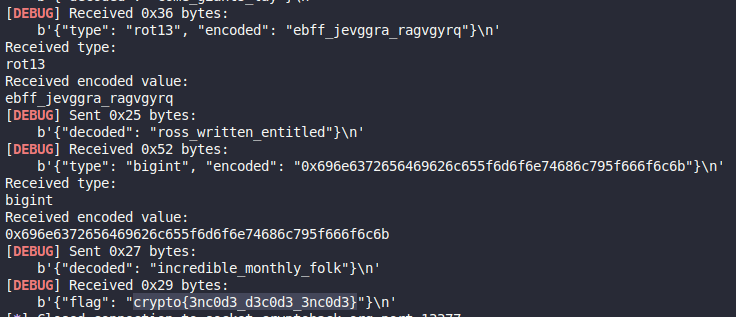
\includegraphics[width=0.8\linewidth]{Images/Encode/encode_chall_result.png}
                
                % La légende qui apparaîtra sous l'image.
                \caption{Ceci est le schéma explicatif de notre méthode.}
                
                % L'étiquette pour y faire référence plus tard.
                \label{fig:encodeChallRes}
            \end{figure}

            Après cent requêtes valides, le \textit{flag} \textit{crypto\{3nc0d3\_d3c0d3\_3nc0d3\}} a été obtenu, permettant la validation du challenge.
            
    \subsection{Xor (Lemur)}
            La deuxième sous-partie de la catégorie \textit{General} est consacrée à 
        l'opération XOR (ou exclusif), un concept fondamental en cryptographie 
        constituant l'une des briques de base de nombreux algorithmes de chiffrement. 
        Sa simplicité de mise en œuvre et ses propriétés mathématiques uniques en font 
        un outil puissant pour manipuler l'information.
        
        Comprendre le fonctionnement du XOR est une étape cruciale, car il se situe à la 
        frontière entre l'opération logique et le chiffrement. L'une de ses propriétés 
        essentielles est sa réversibilité: appliquer deux fois la même clé XOR 
        à une donnée permet de retrouver la donnée originale ($A \oplus K \oplus K = A$). 
        Cette caractéristique est au cœur de son utilisation dans des chiffrements à flux 
        comme le One-Time Pad.
        
        Nous avons décidé de présenter le challenge le plus représentatif de cette partie, 
        nommé \textit{Lemur XOR}.
        
        \subsubsection{Objectifs}
        
        Le but de ce challenge est de retrouver le \textit{flag}, à partir de deux images fournies : \texttt{lemur.png} et \texttt{flag.png}. L'énoncé nous apprend que ces deux images ont été chiffrées avec l'opération XOR en utilisant la même clé secrète.

        \begin{figure}[htbp] % L'environnement figure global
            \centering % Pour centrer le bloc des deux images
        
            \begin{minipage}{0.48\textwidth}
                \centering
                
\includegraphics[width=\linewidth]{Images/Lemur/flag.png} % Première image
            \end{minipage}
            \hfill % Ajoute un espace horizontal flexible entre les images
            \begin{minipage}{0.48\textwidth}
                \centering
                
\includegraphics[width=\linewidth]{Images/Lemur/lemur_ed66878c338e662d3473f0d98eedbd0d.png} % Deuxième image
            \end{minipage}
        
            \caption{Ceci est la légende commune pour les deux images.}
            \label{fig:deux-images}
        \end{figure}
        
        Le principe de résolution repose sur le fait qu'appliquer deux fois un XOR avec la même clé annule l'opération. En effectuant un XOR entre les deux images chiffrées que nous possédons, la clé secrète commune s'élimine, ne laissant que le résultat du XOR entre les deux images originales. C'est sur cette image combinée que le \textit{flag} devrait devenir visible.
        
        \subsubsection{Méthode}
        
        Pour résoudre ce challenge, nous avons utilisé un script en Python avec la bibliothèque de manipulation d'images \textbf{Pillow}. Nous avons commencé par charger les deux images, \texttt{lemur.png} et \texttt{flag.png}. Conformément aux instructions, nous avons appliqué l'opération XOR pixel par pixel sur les valeurs de couleur RVB, et non sur les fichiers entiers.
        
        Nous avons donc parcouru les deux images simultanément et calculé la nouvelle valeur de chaque pixel en effectuant un XOR sur ses composantes rouge, verte et bleue. Nous avons ensuite utilisé ces nouveaux pixels pour construire une image de sortie de mêmes dimensions que nous avons sauvegardée.
        
        \subsubsection{Résultat}
        
            \begin{figure}[H]
                \centering
                % La commande pour insérer l'image.
                % 'width=0.8\linewidth' signifie que l'image fera 80% de la largeur du texte.
                
\includegraphics[width=0.8\linewidth]{Images/Lemur/xored_result.png}
                
                % La légende qui apparaîtra sous l'image.
                \caption{Ceci est le schéma explicatif de notre méthode.}
                
                % L'étiquette pour y faire référence plus tard.
                \label{fig:encodeChallRes}
            \end{figure}

        
        
    \subsection{Data formats (Transparency)}
        \subsubsection{Introduction}
            Le challenge s'appuie sur le principe de \emph{Certificate Transparency} (CT), une mesure de sécurité imposée aux Autorités de Certification (CA) pour garantir la transparence dans la délivrance des certificats TLS.
            
            Un certificat TLS (souvent appelé certificat SSL ou certificat numérique) est un document électronique qui remplit deux fonctions principales :
            \begin{itemize}
                \item Authentifier l'identité d'un site web (ou d'un domaine) auprès des clients (navigateurs, applications).
                \item Établir une connexion chiffrée (TLS) entre le client et le serveur, garantissant la confidentialité et l'intégrité des données échangées.
            \end{itemize}
        
            Un \emph{CT log} est une base de données publique, append-only (où l'on ne peut qu'ajouter des entrées) dans laquelle les certificats émis par les CA sont enregistrés. Aujourd'hui, les principales CA doivent publier (ou « soumettre ») chaque certificat qu'elles émettent dans au moins deux logs CT publics pour qu'il soit accepté et reconnu comme valide par les navigateurs modernes.
        
            Ces logs sont « audités » et surveillés : chacun peut vérifier les entrées, détecter des certificats inattendus, ou vérifier la cohérence de la structure interne (par exemple via un arbre de Merkle) pour s'assurer qu'on ne cache pas d'entrées.
            
        \subsubsection{Objectifs}
            L'objectif de ce challenge est double :
            \begin{enumerate}
                \item Retrouver le sous-domaine de \texttt{cryptohack.org} qui utilise la même clé publique que celle fournie dans le fichier \texttt{transparency.pem} dans son certificat TLS.
                \item En visitant ce sous-domaine, obtenir le \emph{flag}.
            \end{enumerate}
            
            À travers ce challenge, les objectifs pédagogiques sont :
            \begin{itemize}
                \item Comprendre le fonctionnement d’un certificat TLS et sa structure (clé publique, signature, chaîne de confiance, etc.).
                \item Découvrir le système des \emph{Certificate Transparency logs}, bases de données publiques des certificats valides.
                \item Apprendre à faire correspondre une clé publique à un certificat.
                \item Utiliser des outils d’investigation SSL/TLS et de recherche de certificats.
            \end{itemize}
        
        \subsubsection{Méthode}
            \paragraph{Étape 0 : Compréhension du format PEM}
            \begin{itemize} 
            \item Le fichier fourni est au format PEM (Privacy-Enhanced Mail), un format standard pour les clés cryptographiques qui utilise l'encodage Base64. Exemple (clé publique fournie) :
            
\item\begin{verbatim}
-----BEGIN PUBLIC KEY-----
MIIBIjANBgkqhkiG9w0BAQEFAAOCAQ8AMIIBCgKCAQEAuYj06m5q4M8SsEQwKX+5
NPs2lyB2k7geZw4rP68eUZmqODeqxDjv5mlLY2nz/RJsPdks4J+y5t96KAyo3S5g
mDqEOMG7JgoJ9KU+4HPQFzP9C8Gy+hisChdo9eF6UeWGTioazFDIdRUK+gZm81c1
iPEhOBIYu3Cau32LRtv+L9vzqre0Ollf7oeHqcbcMBIKL6MpsJMG+neJPnICI36B
ZZEMu6v6f8zIKuB7VUHAbDdQ6tsBzLpXz7XPBUeKPa1Fk8d22EI99peHwWt0RuJP
0QsJnsa4oj6C6lE+c5+vVHa6jVsZkpl2PuXZ05a69xORZ4oq+nwzK8O/St1hbNBX
sQIDAQAB
-----END PUBLIC KEY-----
\end{verbatim}
\end{itemize}

            \paragraph{\textbf{Étape 1 : Analyse du problème initial.}} 
            \begin{itemize} 
            \item On cherche à comprendre comment relier une empreinte SHA-256 à un certificat TLS complet et comment extraire la clé publique d'un certificat. 
            \item \textbf{Constatations :} 
            \begin{enumerate} 
            \item Un certificat TLS X.509 contient une clef publique encapsulée. 
            \item La représentation DER est la base sur laquelle on calcule l'empreinte SHA-256 utilisée par certains services (par ex. crt.sh avec le paramètre spkisha256). 
            \item Les formats PEM (texte Base64) et DER (binaire) sont des représentations interchangeables de la même information. 
            \end{enumerate} 
            \end{itemize}
            
            \paragraph{\textbf{Étape 2 : Conception du script pas à pas.}}~\\
            
            Les objectifs du script sont : 
            \begin{enumerate} 
            \item Générer l'empreinte SHA-256 de la clé publique fournie. 
            \item Interroger les CT logs (par exemple via \texttt{crt.sh}) pour retrouver les certificats. 
            \item Télécharger le certificat complet (PEM) identifié dans les logs. 
            \item Extraire le nom de domaine du certificat. 
            \item Accéder et récupérer le flag. 
            \end{enumerate}
            
        
        \subsubsection{Résultat}
            L'exécution du processus a produit les résultats suivants : 
            \begin{itemize} 
            \item \textbf{Empreinte (SHA-256):} 
            \begin{verbatim}
            29ab37df0a4e4d252f0cf12ad854bede59038fdd9cd652cbc5c222edd26d77d2
            \end{verbatim} 
            \item \textbf{Sous-domaine identifié :} 
            \begin{verbatim}
            thetransparencyflagishere.cryptohack.org
            \end{verbatim} 
            \item \textbf{Flag obtenu :} 
            \begin{verbatim}
            crypto{thx_redpwn_for_inspiration}
            \end{verbatim} 
            \end{itemize}


\section{Diffie-Hellman}
    \subsection{Objectifs généraux de la catégorie du challenge}
    % Contenu à rédiger ici
    
    \subsection{Man in the middle (Export grade)}
    % Contenu à rédiger ici

\section{RSA}
    \subsection{Objectifs généraux de la catégorie du challenge}
    % Contenu à rédiger ici

% --- FIN DU DOCUMENT ---

\end{document}
